\documentclass[Arkitektur/System_main.tex]{subfiles}
\begin{document}
\subsection{Scenerier}
I dette afsnit beskrives systemets funktionalitet og adfærd, som tages udgangspunkt i distributionerne angivet tidligere. For at illustrere systemets adfærd bruges sekvensdiagrammer, som beskriver sammenspillet mellem aktører, applikation og database. 

\subsubsection{Oprettelse af bruger}
For at kunne anvende CarnGo applikation må brugeren oprette en profil. Brugerens information gemmes i databasen ved oprettelse. 
\begin{figure}[H]
    \centering
    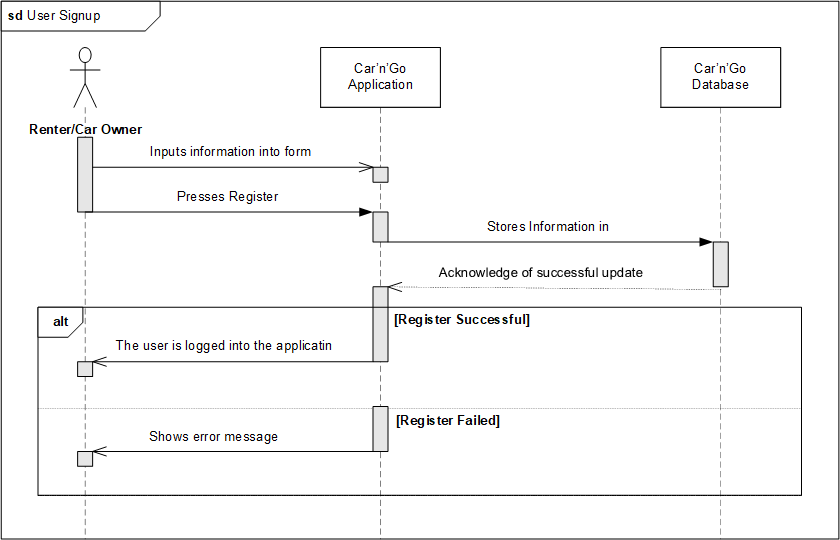
\includegraphics[width=\textwidth]{Arkitektur/Softwarearkitektur/User_Signup/graphics/UserSignupSD.png}
    \caption{Her ses et skevens diagram for samspillet mellem lejer/udlejer, CarnGo applikationen samt databasen.}
    \label{fig:UserSignUpSD}
\end{figure}

\subsubsection{Redigering/Fjernelse af bruger}
Alle registrerede brugere i systemet har tilknyttet visse informationer, som identificerer dem som person. Det skal være muligt at ændre brugerinformationer, samt slette brugeren, hvis den ikke ønskes længere - brugeren skal være logget ind i applikation for at kunne lave ændringer. 
\begin{figure}[H]
    \centering
    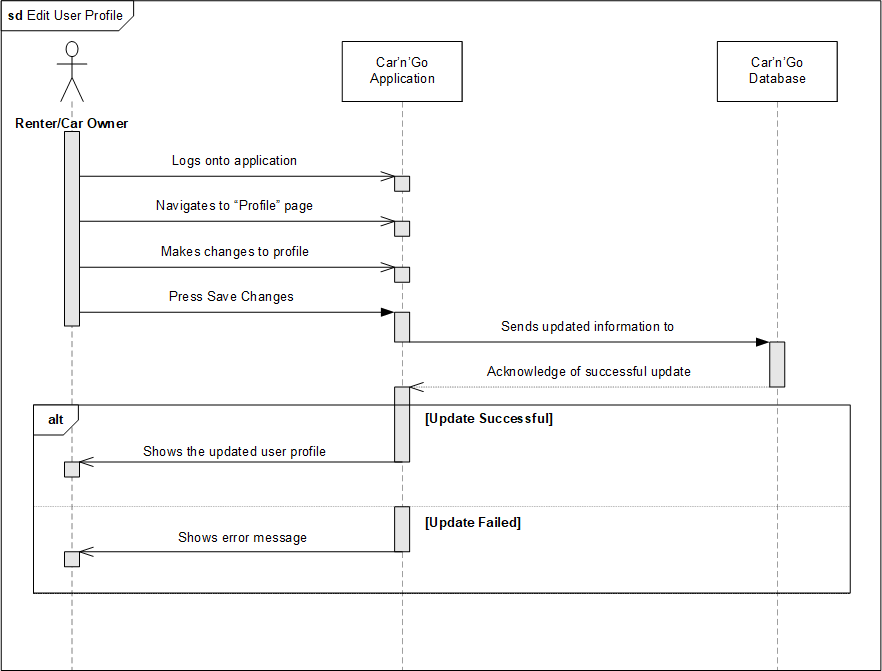
\includegraphics[width=1\textwidth]{Arkitektur/Softwarearkitektur/Edit_user_profile/graphics/SystemSD_ProfilerSD.png}
    \caption{Sekvensdiagram for redigering og fjernelse af en brugerprofil. }
    \label{fig:EditUserSD}
\end{figure}

\subsubsection{Oprettelse af Bilprofil}
En bilprofil repræsentere alt information omkring den bil som udlejes. En bruger med udlejerrettigheder skal have mulighed for at oprette en bilprofil. En bruger med lejerrettigheder har ikke mulighed for at oprette bilprofiler. 
\begin{figure}[H]
    \centering
    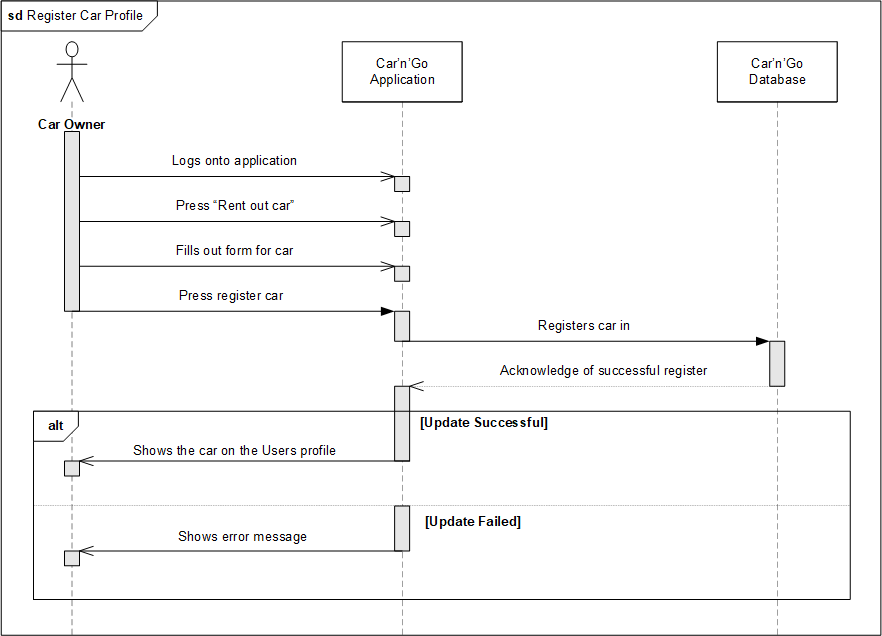
\includegraphics[width=1\textwidth]{Arkitektur/Softwarearkitektur/Car_registration/graphics/RegisterCarSD.png}
    \caption{Her ses et sekvensdiagram for samspillet mellem udlejer, applikation og database. }
    \label{fig:RegisterCarProfileSD}
\end{figure}

\subsubsection{Redigering/Fjernelse af Bilprofil}
Det skal være muligt at ændre eller fjerne en allerede oprettet bilprofil - brugeren med udlejerrettigheder skal være logget ind i applikation for at kunne lave ændringer. 
\begin{figure}[H]
    \centering
    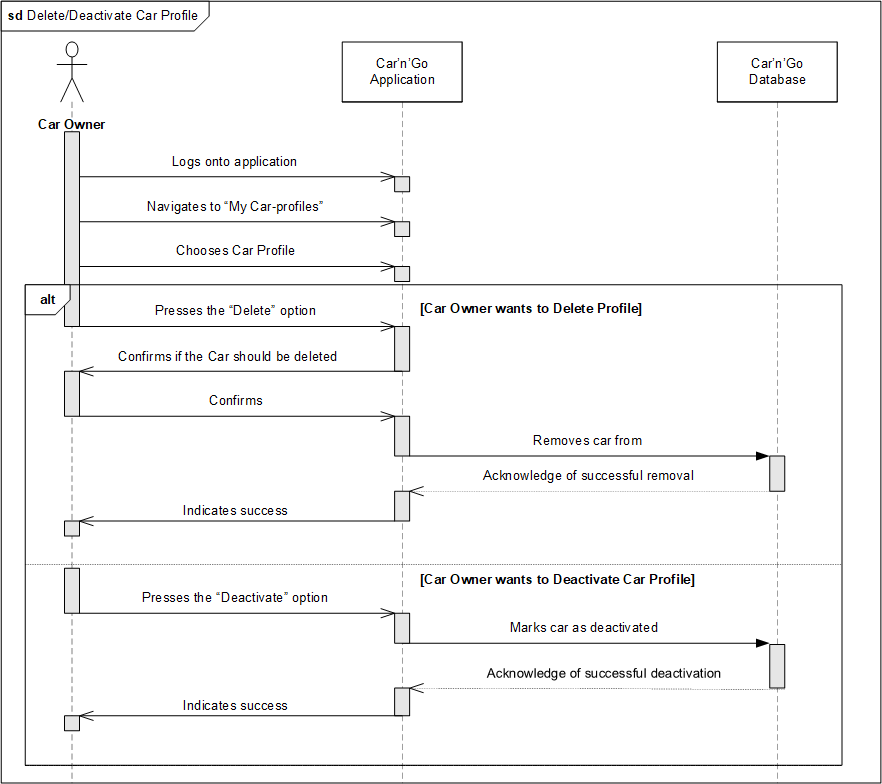
\includegraphics[width=1\textwidth]{Arkitektur/Softwarearkitektur/Car_registration/graphics/DeleteCarProfileSD.png}
    \caption{Her ses sekvensdiagrammet for fjernelsen af en bilprofil, som viser samspillet mellem udlejer, applikation og database. }
    \label{fig:DeleteCarProfileCD}
\end{figure}

\subsubsection{Søgning af udlejningsbil}
Når en lejer ønsker at leje en bil, så skal han søge efter en i applikationens katalog, hvor udlejere har sat dem til leje. 
\begin{figure}[H]
    \centering
    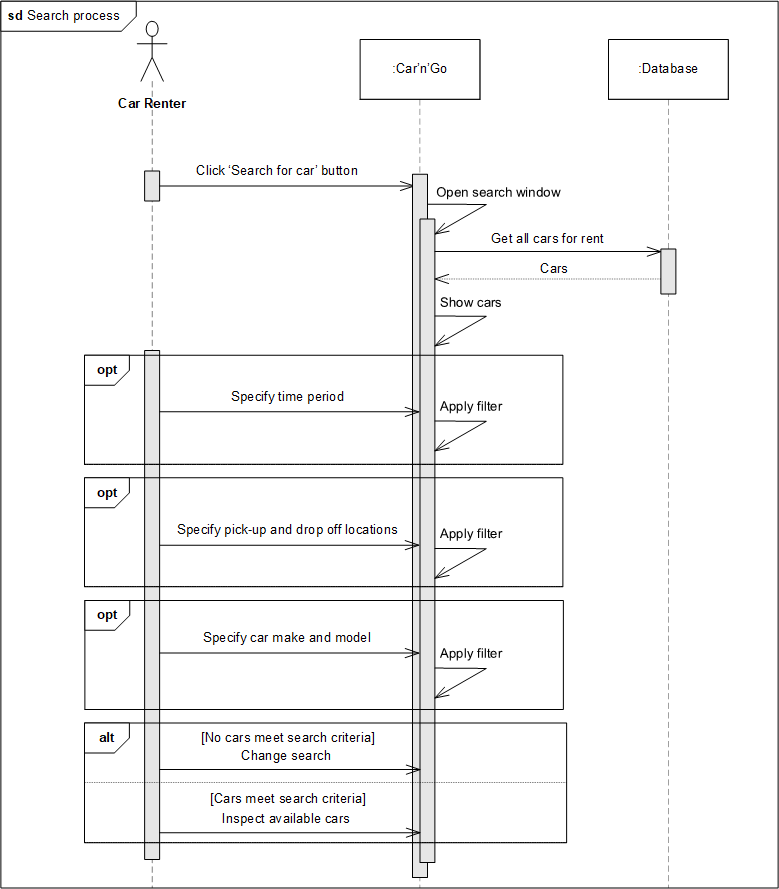
\includegraphics[width=1\textwidth]{Arkitektur/Softwarearkitektur/Searching/graphics/Search_Process_SD.png}
    \caption{Sekvensdiagram for søgning efter biler til leje. }
    \label{fig:SearchProcessSD}
\end{figure}

\subsubsection{Håndtering af udlejningsproces}
Efter at lejer har søgt i applikationens katalog, og har fundet en bil, som lejer ønsker at leje, så starter udlejningsprocessen. Dette realiseres med 3 trin:
\begin{enumerate}
    \item Lejer anmoder udlejer om billeje 
    \item Udlejer godkender/forkaster anmodning om billeje 
    \item [Valgfri] Lejer tager kontakt til udlejer i forhold til udveksling af bil. 
\end{enumerate}
\begin{figure}[H]
    \centering
    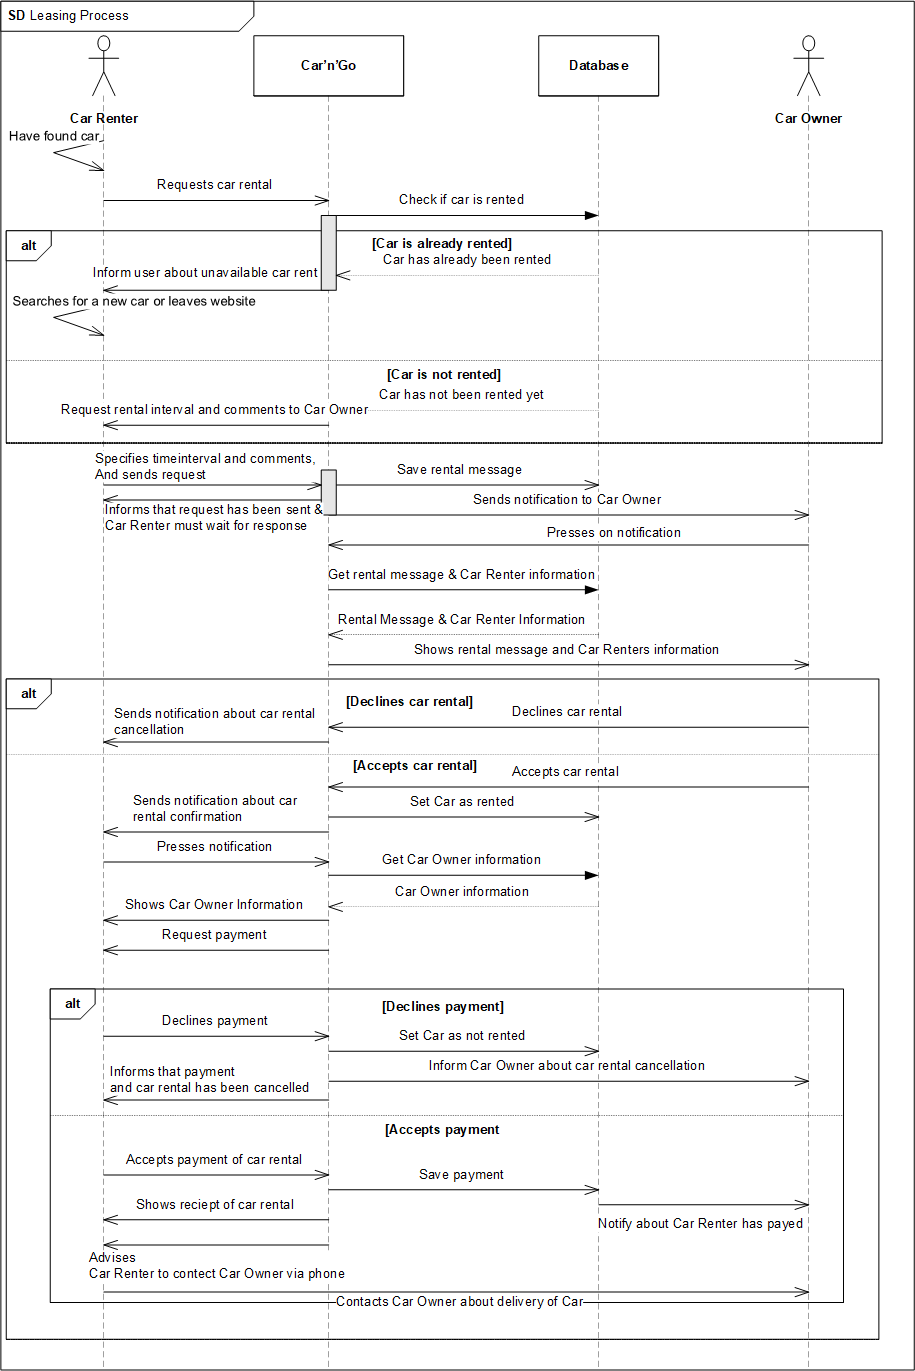
\includegraphics[width=1.1\textwidth]{Arkitektur/Softwarearkitektur/Leasing/graphics/Leasing_processSD.png}
    \caption{Sekvensdiagram for håndtering af udlejningsprocessen.}
    \label{fig:Leasing_processCD}
\end{figure}
\end{document}